\section{Esercizio 18}
\textit{\textbf{Descrizione:} Confrontare i codici degli esercizi $14-17$ per approssimare la funzione $f(x) = sin(x)$ sulle ascisse $x_{i} = i \pi/n, i = 0, 1, \cdots , n,$ per $n = 1, 2, \cdots, 10$. Graficare l'errore massimo di approssimazione verso n (in semilogy), calcolato su una griglia uniforme di 10001 punti nell'intervallo $[0, \pi]$.}\newline
\noindent\emph{Soluzione: }\newline
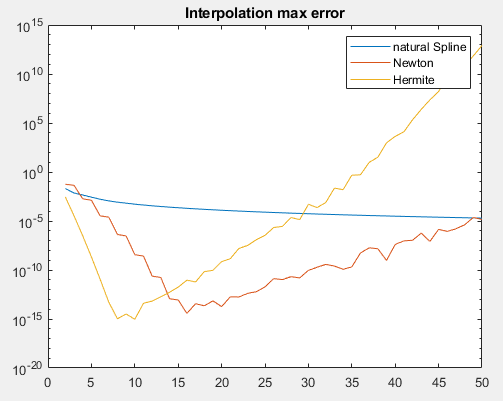
\includegraphics[width=1.3\linewidth]{img/errorInterp.png}